\documentclass[professionalfonts]{beamer}
\newif\ifita
\itatrue % comment out to hide answers
\itafalse
\usepackage[familydefault,light]{Chivo} 
\usepackage[T1]{fontenc}
\usenavigationsymbolstemplate{}
\usepackage[]{hyperref}
\usepackage{tikz,pgf,pgfarrows,pgfnodes,pgfbaseimage}
\graphicspath{{./Pics/}}
\usetikzlibrary{shapes}
\usepackage{setspace}
\newcommand{\evi}[1]{{\colorbox{yellow!50}{{#1}}}}
\newcommand{\exe}[1]{{\color{black!50}{{#1}}}}
\newcommand{\kw}[1]{{\colorbox{black!30}{\color{white}{#1}}}}
\tikzstyle{nd}=[circle,draw=black,thick,minimum size=.8cm,inner sep=1pt]
\setbeamercovered{transparent}
\usetheme{Singapore}
\tikzstyle{nodo}=[ellipse,draw=black!60,fill=black!10,line width=.7pt,minimum width=.7cm,minimum height=.4cm]
\usecolortheme[named=gray]{structure}
\setbeamercolor{block title}{bg=black!20,fg=black}
\setbeamercolor{block body}{bg=black!10,fg=black}

%%%%%%%%%%%%%%%%%%%%%
\ifita
\title{Algoritmi Numerici (Parte IV)}
\subtitle{[Lezione 0] Interpolazione}
\else
\title{Numerics (Part IV)}
\subtitle{[Lecture 0] Interpolation}
\fi
\date{}
\author{Alessandro Antonucci\\{\tt alessandro.antonucci@supsi.ch}}
%%%%%%%%%%%%%%%%%%%%%%%%%%%%
\begin{document}
\maketitle
\frame{\frametitle{\ifita Alcuni esempi \else Some examples\fi}
\begin{itemize}
\item \ifita Registro l'intensit\`a di precipitazione ogni 10 minuti \else Recording rainfall intensity every 10 minutes\fi
\item \ifita Intensit\`a alle 13:27? \else Intensity at 1:27pm? \fi
\item \ifita Quantit\`a di pioggia caduta in un intervallo di tempo? \else Total rainfall in a given time window \fi
\end{itemize}
\begin{center}
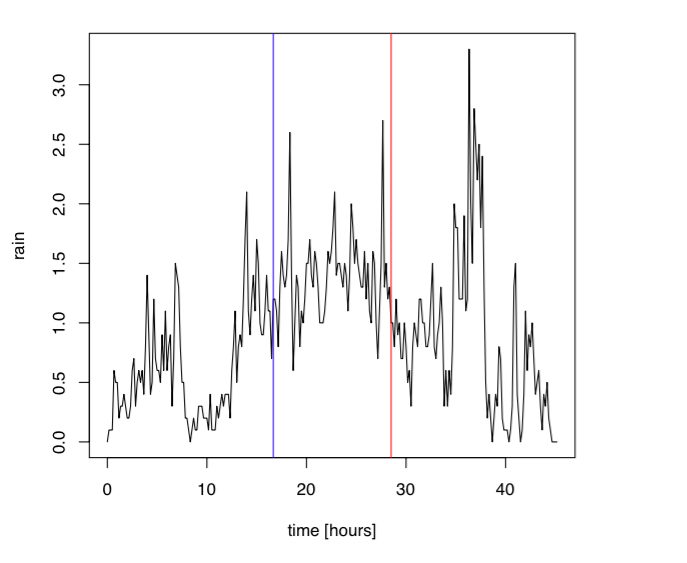
\includegraphics[width=10cm,height=4cm]{figinterp1}
\vskip 2mm
$I(t=13:27)=? \quad \quad$ 
$\int_{T_i}^{T_f} I(t) \mathrm{d}t=?$
\end{center}}
\frame{\frametitle{\ifita Alcuni esempi (ii)\else Some examples (ii)\fi}
\begin{itemize}
\item \ifita Un robot deve passare per un certo numero di punti \else Robot required to cross a number of points \fi
\item \ifita Raggio di curvatura traiettorie limitato \else Curvature in trajectories has a miinimum \fi
\item \ifita Che strada fare? \else Best path? \fi
\end{itemize}
\begin{center}
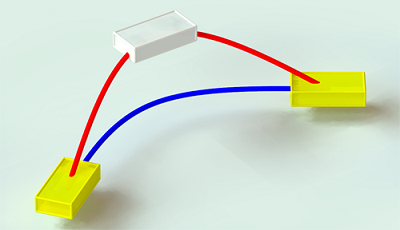
\includegraphics[width=10cm,height=4cm]{figinterp2}
\end{center}}

\frame{\frametitle{\ifita Alcuni esempi \else Some examples \fi (iii)}
\begin{itemize}
\item Design, \ifita animazione \else animation \fi (2D, 3D), $\ldots$
\end{itemize}
\begin{center}
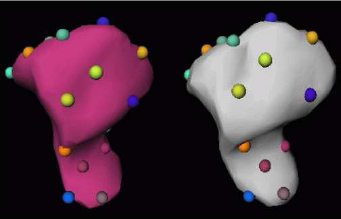
\includegraphics[width=5cm,height=4cm]{figinterp3}
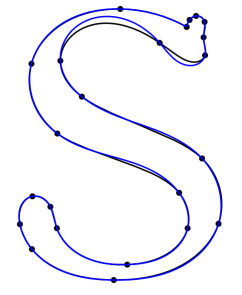
\includegraphics[width=5cm,height=4cm]{figinterp4}
\end{center}}

\frame{\frametitle{Connecting the dots}
\begin{center}

\includegraphics[width=10cm,height=6cm]{jobs}
\end{center}}

\setbeamercovered{}
\frame{\frametitle{Connecting the dots}
\begin{tikzpicture}[rotate=0,domain=-5:10,xscale=.7]
\filldraw [black] (-5,1) circle (1.5pt);
\filldraw [black] (-4,0) circle (1.5pt);
\filldraw [black] (-3,-2) circle (1.5pt);
\filldraw [black] (-2,0) circle (1.5pt);
\filldraw [black] (-1,1) circle (1.5pt);
\filldraw [black] (0,0) circle (1.5pt);
\filldraw [black] (1,1) circle (1.5pt);
\filldraw [black] (2,0) circle (1.5pt);
\filldraw [black] (3,0) circle (1.5pt);
\filldraw [black] (4,1) circle (1.5pt);
\filldraw [black] (5,0) circle (1.5pt);
\filldraw [black] (6,-1) circle (1.5pt);
\filldraw [black] (7,0) circle (1.5pt);
\filldraw [black] (8,1) circle (1.5pt);
\filldraw [black] (9,0) circle (1.5pt);
\filldraw [black] (10,-1) circle (1.5pt);
{\onslide<2->
\draw[color=blue] plot[id=pa,domain=-5:-4] function{1-(x+5)**2};
\draw[color=blue] plot[id=pb,domain=-4:-3] function{-2*(x+4)};
\draw[color=blue] plot[id=pc,domain=-3:-2] function{4*x*x+22*x+28};
\draw[color=blue] plot[id=pd,domain=-2:-1] function{-(x+2)*(5*x+4)};
\draw[color=blue] plot[id=pe,domain=-1:0] function{3*x*x+2*x};
\draw[color=blue] plot[id=pf,domain=0:1] function{x-x*(x-1)+.5*x*(x-1)*(x-2)-.125*x*(x-1)*(x-2)*(x-3)};
\draw[color=blue] plot[id=pg,domain=1:2] function{x-x*(x-1)+.5*x*(x-1)*(x-2)-.125*x*(x-1)*(x-2)*(x-3)};
\draw[color=blue] plot[id=ph,domain=2:3] function{x-x*(x-1)+.5*x*(x-1)*(x-2)-.125*x*(x-1)*(x-2)*(x-3)};
\draw[color=blue] plot[id=pi,domain=3:4] function{x-x*(x-1)+.5*x*(x-1)*(x-2)-.125*x*(x-1)*(x-2)*(x-3)};
\draw[color=blue] plot[id=pl,domain=4:5] function{x-x*(x-1)+.5*x*(x-1)*(x-2)-.125*x*(x-1)*(x-2)*(x-3)};
\draw[color=blue] plot[id=pm,domain=9:10] function{(.0000*(x-9)**3+.8038*(10-x)**3)/6+(-1)*(x-9)+(0-.8038/6)*(10-x)};
\draw[color=blue] plot[id=pn,domain=8:9] function{(.8038*(x-8)**3-3.2153*(9-x)**3)/6+(0-.8038/6)*(x-8)+(1+3.2153/6)*(9-x)};
\draw[color=blue] plot[id=po,domain=7:8] function{(-3.2153*(x-7)**3+.0574*(8-x)**3)/6+(1+3.2153/6)*(x-7)+(-.0574/6)*(8-x)};
\draw[color=blue] plot[id=pp,domain=6:7] function{(.0574*(x-6)**3+2.9856*(7-x)**3)/6+(0-.0574/6)*(x-6)+(-1-2.9856/6)*(7-x)};
\draw[color=blue] plot[id=pq,domain=5:6] function{(2.9856*(x-5)**3+.0*(6-x)**3)/6+(-1-2.9856/6)*(x-5)+(0-0)*(6-x)};}
\end{tikzpicture}
}


\frame{\frametitle{\ifita (Algoritmi di) Interpolazione \else Interpolation Algorithms\fi}
\begin{block}{Input}
\begin{itemize}
\item \ifita Data una serie di $n+1$ punti \else Given a set of $n+1$ points \fi $\{ (x_i,y_i) \}_{i=0}^n$
\item \ifita Tali che \else Such that \fi $x_{i+1}>x_i$ $\forall i$ \color{gray}{\ifita (da sx a dx, mai stessa ascissa) \else (from left to right, no same $x$ \fi)}
\end{itemize}
\end{block}
\begin{block}{Output}
\begin{itemize}
\item \ifita Trovare una funzione \else Finding function \fi $f(x)$ \ifita definita tra \else defined between \fi $x_0$ \ifita e \else and \fi $x_{n}$
\item \ifita Tale che \else Such that \fi $f(x_i)=y_i$ {$\forall i=0,1,\ldots,n$ \color{gray}{($f$ \ifita passa per i punti \else touches the points \fi)} }
\item \ifita $f$ continua \else continuous $f$ \fi {\color{gray}{(\ifita opzionalmente anche derivata/e continua/e \else optionally also derivatives continuous \fi)}}
\end{itemize}
\end{block}
\vskip 2mm
\begin{center}
\it \ifita Algoritmi diversi interpoleranno i punti in maniera diversa\\
non posso dire se un'interpolazione \`e meglio di un'altra \else 
Different algorithms produce different interpolations\\ in general cannot say which one is better
\fi
\end{center}}

\frame{\frametitle{\ifita Il pi\`u semplice algoritmo di interpolazione \else The simplest interpolation algorithm \fi}
\begin{itemize}
\item \ifita Sp-line lineare: congiungo coppie di punti consecutivi con segmenti di retta
\else
Linear sp-line: consecutive pairs of points connected by straight lines
\fi
{\onslide<1->\item \ifita Vantaggi: banale da implementare \else Pros: easy to implement \fi
$$f(x)=y_j+\frac{y_{j+1}-y_{j}}{x_{j+1}-x_{j}} (x-x_j) \quad \mathrm{if} \quad x \in [x_j,x_{j+1}]$$}
{\onslide<1->\item \ifita Svantaggi: derivata discontinua (punti angolosi) \else Cons: discontinuous derivative (sharp points)\fi}
\end{itemize}
\begin{center}
{\onslide<1->
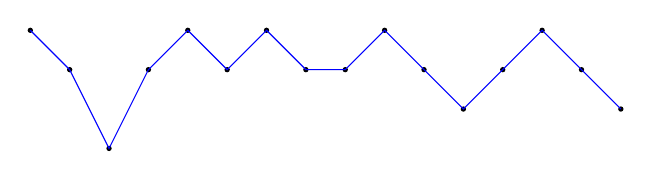
\begin{tikzpicture}[rotate=0,domain=-5:10,scale=.5]
\filldraw [black] (-5,1) circle (1.5pt);
\filldraw [black] (-4,0) circle (1.5pt);
\filldraw [black] (-3,-2) circle (1.5pt);
\filldraw [black] (-2,0) circle (1.5pt);
\filldraw [black] (-1,1) circle (1.5pt);
\filldraw [black] (0,0) circle (1.5pt);
\filldraw [black] (1,1) circle (1.5pt);
\filldraw [black] (2,0) circle (1.5pt);
\filldraw [black] (3,0) circle (1.5pt);
\filldraw [black] (4,1) circle (1.5pt);
\filldraw [black] (5,0) circle (1.5pt);
\filldraw [black] (6,-1) circle (1.5pt);
\filldraw [black] (7,0) circle (1.5pt);
\filldraw [black] (8,1) circle (1.5pt);
\filldraw [black] (9,0) circle (1.5pt);
\filldraw [black] (10,-1) circle (1.5pt);
{\onslide<1->
\draw[color=blue] (-5,1) -- (-4,0) -- (-3,-2) -- (-2,0) -- (-1,1) -- (0,0) -- (1,1) -- (2,0) -- (3,0) -- (4,1) -- (5,0) -- (6,-1) -- (7,0) -- (8,1) -- (9,0) -- (10,-1);}
\end{tikzpicture}}
\end{center}}

\frame{\frametitle{\ifita Interpolazione polinomiale \else Polynomial interpolation\fi}
\begin{itemize}
{\onslide<1->\item 2 \ifita punti \else points \fi? \ifita Passa una (e solo una) retta (= pol grado 1)\else Connected by one (and only one) straight line (polynomial of degree 1)\fi}
{\onslide<2->\item 3 \ifita punti \else points \fi? \ifita Passa una (e solo una) parabola (= pol grado 2)\else Connected by one (and only one) parabolic curve (polynomial of degree 2)\fi}
{\onslide<3->\item 4 \ifita punti \else points \fi? \ifita Passa una (e solo una) cubica (= pol grado 3)\else Connected by one (and only one) cubic curve (polynomial of degree 3)\fi}
{\onslide<3->\item $\ldots$}
{\onslide<3->\item $n+1$ \ifita punti \else points \fi? \ifita Passa una (e solo una) funzione di grado $n$ \else Connected by one (and only one) function of degree $n$\fi}
{\onslide<3-> \item \ifita  Vantaggi: (infinitamente) derivabile \else Pros: infinitely many derivatives \fi}
\end{itemize}
\begin{center}
\begin{tikzpicture}[rotate=0,domain=0:5,scale=1]
{\onslide<1->\filldraw [black] (0,0) circle (1.5pt); \filldraw [black] (1,2) circle (1.5pt);}
{\onslide<1-1>\draw[color=blue] plot[id=pollin,domain=-.2:1.2] function{2*x};}
{\onslide<2-2>\filldraw [black] (2,1) circle (1.5pt);}
{\onslide<2-2>\draw[color=red] plot[id=polquad,domain=-.2:2.2] function{-1.5*x*x+3.5*x};}
{\onslide<3->\filldraw [black] (3,0) circle (1.5pt);}
{\onslide<3-3>\draw[color=green] plot[id=polcub,domain=-.2:3.2] function{0.5*x*x*x-3*x*x+4.5*x};}
\end{tikzpicture}
\end{center}}


\frame{\frametitle{\ifita Algoritmo per Interpolazione Polinomiale \else Algorithm for Polynomial Interpolation\fi}
\begin{itemize}
\item \ifita Generico polinomio di grado $n$ \else Generic $n$-degree polynomial \fi: $p_n(x)=\sum_{i=0}^n a_i x^i$
\item \ifita Dipende da $n+1$ parametri (incognite) \else $n+1$ (unknown) parameters \fi
\item \ifita Imponendo il passaggio per gli $n+1$ punti,\else Requiring the $n+1$ points to be crossed\fi \\
\ifita trovo sistema quadrato \else linear system \fi $(n+1) \times (n+1)$:
\begin{center}
\vskip 1mm
$\begin{array}{ccccc}
a_0 & a_1 & a_2 & \ldots &a_n\\
\end{array}$
\vskip 1mm$
\begin{array}{|ccccc|c|}
\hline
1 & x_0 & x_0^2 & \ldots & x_0^n & y_0\\ 
1 & x_1 & x_1^2 & \ldots & x_1^n & y_1\\
&&\ldots&\ldots&&\\
1 & x_n & x_n^2 & \ldots & x_n^n&y_n\\
\hline
\end{array}$
\end{center}
\vskip 2mm
\item \ifita Possso interpolare $n+1$ punti con complessit\`a cubica \else Cubic algorithm for polynomial interpolation \fi
\end{itemize}}

\frame{\frametitle{\ifita Un Algoritmo Migliore per Interpolazione Polinomiale \else A better algorithm for polynomial interpolation\fi}
\begin{itemize}
\item \ifita Forma alternativa per polinomio, es. \else Alternative formulation for polynomials, ex. \fi 
$p_3(x)=c_0+c_1 (x-x_0) + c_2(x-x_0)(x-x_1)+c_3(x-x_0)(x-x_1)(x-x_2)$
\item $p_n(x)=\sum_{i=0}^n c_i \left[ \prod_{j=0}^{i-1} (x-x_j) \right] $
\item \ifita Impongo passaggio per gli $n+1$ punti: \else Forcing the polynomial to cross the $n+1$ points \fi
\vskip 5mm
\begin{center}
$\begin{array}{|ccccc|c|}
\hline
1 & 0 & 0 & \ldots & 0 & y_0\\ 
1 & x_1-x_0 & 0 & \ldots & 0 & y_1\\
&&\ldots&\ldots&&\\
1 & x_n-x_0 & (x_n-x_0)(x_n-x_1) & \ldots & \prod_{j=0}^{n-1} (x_n-x_j)&y_n\\
\hline
\end{array}$
\end{center}
\vskip 3mm
\item \ifita Sistema triangolare (dopo swaps), risolvo in $O(n^2)$
\else
Triangular system (after swaps), $O(n^2)$ solution!
\fi
\end{itemize}}
\end{document}
